\documentclass[class=minimal,border=0pt]{standalone}
\usepackage{tikz}
\usetikzlibrary{arrows.meta}
\begin{document}
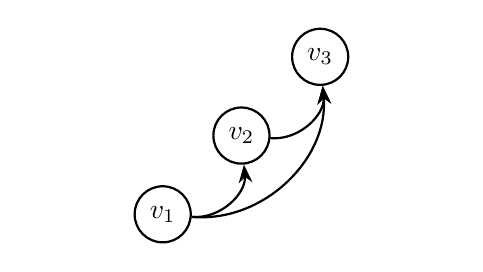
\begin{tikzpicture}
\begin{scope}[every node/.style={circle,thick,draw}]
    \node (2) at (1.5 ,1  )  {$v_1$};
    \node (3) at (2.5 ,2  )  {$v_2$};
    \node (4) at (3.5 ,3  )  {$v_3$};
\end{scope}

\begin{scope}[every node/.style={circle,thick,draw,white}]
    \node[draw=none] (1) at (0   ,1.5)  {.};
    \node[draw=none] (5) at (5   ,2.5)  {.};
\end{scope}

\begin{scope}[>={Stealth[black]},
              every node/.style={fill=white,circle},
              every edge/.style={draw}]
    %\path [->] (1) edge[bend left =50,thick] (2);
    %\path [->] (1) edge[bend left =40,dashed] (3);
    %\path [->] (1) edge[bend left =30,dashed] (4);

    %\path [->] (2) edge[bend right=30,dashed] (5);
    %\path [->] (3) edge[bend right=40,dashed] (5);
    %\path [->] (4) edge[bend right=50,thick] (5);

    \path [->] (2) edge[bend right=50,thick] (3);
    \path [->] (2) edge[bend right=50,thick] (4);
    \path [->] (3) edge[bend right=50,thick] (4);
\end{scope}
\end{tikzpicture}
\end{document}
